% !TEX root = hw2-robot.tex
\documentclass[a4paper, 12pt, oneside, fleqn]{article}

\usepackage{amsmath, amssymb, amsthm}       % 美國數學學會
\usepackage[CheckSingle, CJKmath]{xeCJK}    % 中文
\usepackage{fontspec}                       % 字型設定
\usepackage{geometry}                       % 版面設定
\usepackage[nocheck]{fancyhdr}              % 頁首頁尾
\usepackage{color}                          % 顏色
\usepackage[x11names]{xcolor}               % 更多顏色
\usepackage{datetime2}                      % 日期、時間
\usepackage{listings}                       % 顯示 code 用的
\usepackage{titlesec}                       % 標題格式控制
\usepackage{tikz}                           % 畫圖
\usepackage{enumerate}                      % 列舉環境
\usepackage{enumitem}                       % 自訂列舉環境
\usepackage{ulem}                           % 文字底線、刪除線
\usepackage{graphicx}                       % 插入圖片
\usepackage{multicol}                       % 多欄排版
\usepackage{hyperref}                       % 超連結
\usepackage{subcaption}                     % 子圖
\usepackage{cancel}                         % 取消線
\usepackage{multirow}                       % 表格合併列
\usepackage{float}                          % 浮動物件位置強制
\usepackage{flafter}                        % 浮動物件不得出現在原文位置之前
\usepackage{notomath}                       % Noto 數學字體
\usepackage{booktabs}                       % 表格橫線
\usepackage{tabularx}                       % 自動欄寬
\usepackage{longtable}                      % 跨頁表格
\usepackage{array}                          % 表格欄位格式
\usepackage{microtype}                      % 英文微排版
\usetikzlibrary{arrows.meta, positioning, shapes.geometric, fit, calc, backgrounds}

%%%%%%%%%%%%%%%%%%%%%%%%%%%%%%

\setmainfont{Noto Serif}  % 主要字體

\setmonofont{Menlo}  % 等寬字體

\setCJKmainfont{Noto Serif CJK TC}[  % 中文主要字體
    ItalicFont     = *-Regular, % 中文沒有斜體
    BoldItalicFont = *-Bold,    % 中文沒有斜體
]

\setCJKmonofont{Noto Sans CJK TC}[  % 中文等寬字體
    ItalicFont     = *-Regular, % 中文沒有斜體
    BoldItalicFont = *-Bold,    % 中文沒有斜體
]

\newCJKfontfamily{\kaifont}[
    AutoFakeBold = 2
]{Kaiti TC}

%%%%%%%%%%%%%%%%%%%%%%%%%%%%%%

% 彩色模式
\newcommand{\keywordcolor}{\color{Blue1}}
\newcommand{\identifiercolor}{\color{black}}
\newcommand{\commentcolor}{\color{Red4}}
\newcommand{\stringcolor}{\color{Green4}}

\makeatletter
\lst@CCPutMacro\lst@ProcessOther {"2D}{\lst@ttfamily{-{}}{-{}}}
\@empty\z@\@empty
\makeatother

\lstset{
    language=C++,
    numbers=left,                           % 行號的位置
    numberstyle=\tiny,                      % 行號的字型和大小
    stepnumber=1,                           % 顯示行號的間隔
    numbersep=5pt,                          % 行號跟 code 的距離
    showspaces=false,                       % 顯示空白 (使用特別的底線記號)
    showtabs=false,                         % 顯示 Tab
    showstringspaces=false,                 % 顯示字串的空白
    tabsize=4,                              % Tab 的寬度
    frame=single,                         % adds a frame around the code
    captionpos=b,                           % sets the caption-position to bottom
    breaklines=true,                        % sets automatic line breaking
    breakatwhitespace=false,                % sets if automatic breaks should only happen at whitespace
    escapeinside={\%*}{*)},                 % if you want to add a comment within your code
    morekeywords={*},                       % 自訂的 Keywords
    basicstyle=\footnotesize\ttfamily,      % 基本的字型和大小
    backgroundcolor=\color{white},          % 背景顏色
    keywordstyle=\bfseries\keywordcolor,    % Keywords 的字型
    identifierstyle=\identifiercolor,       % 標示符的字型
    commentstyle=\itshape\commentcolor,     % 註解的字型
    stringstyle=\itshape\stringcolor,       % 字串的字型
    otherkeywords={Vector},       % 其他的 Keywords
}

%%%%%%%%%%%%%%%%%%%%%%%%%%%%%%

% ===== 頁面設定 =====
\geometry{a4paper}                      % A4 紙
% \geometry{includehead}                  % 內文區塊包含頁首，沒有頁尾、旁注
\geometry{headsep=12pt}                  % 頁首與內文距離稍微拉開
\geometry{vmargin=1in, hmargin=1in}     % 上下左右邊界 1 吋

% ===== 行距與段落 =====
\renewcommand{\baselinestretch}{1.2}    % 正文行距 1.2 倍
\setlength{\parskip}{1.5ex}             % 段落間距略增，讓段落清楚分隔
% \setlength{\parindent}{0pt}             % 段落首行縮排，可依喜好調整

% ===== 標題間距 (section) =====
\titlespacing{\section}{0pt}{12pt}{8pt}
\titlespacing{\subsection}{0pt}{8pt}{6pt}
\titlespacing{\subsubsection}{0pt}{6pt}{4pt}

% ===== 表格列高 =====
% \renewcommand{\arraystretch}{1.5}       % 表格列高 1.5 倍
\setlength{\tabcolsep}{1.25ex}          % 表格欄寬


% \titlespacing{\section}{0pt}{12pt}{6pt}
% \titlespacing{\subsection}{0pt}{6pt}{4pt}
% \titlespacing{\subsubsection}{0pt}{4pt}{2pt}

\XeTeXlinebreaklocale "zh"          % 中文自動換行
\XeTeXlinebreakskip = 0pt plus 1pt  % 設定段落之間的距離
\emergencystretch=3em


%%%%%%%%%%%%%%%%%%%%%%%%%%%%%%

\hypersetup{
    colorlinks=true,         % 啟用顏色連結
    linkcolor=red,           % 內部連結顏色
    filecolor=green,         % 檔案連結顏色
    urlcolor=blue,           % 網址顏色
    pdfborder={0 0 1}        % 設定邊框樣式（0 0 1 表示只有底部有邊框）
}

\setcounter{tocdepth}{2}
\setcounter{secnumdepth}{3}

\tikzset{
    flow/.style={draw, rounded corners=2pt, align=center, minimum height=8mm,
            text width=25mm, fill=blue!5},
    layer/.style={draw, rounded corners=2pt, align=center, minimum height=9mm,
            text width=31mm, fill=gray!8},
    arrow/.style={-{Latex[length=2.2mm]}, thick},
    dashedarrow/.style={-{Latex[length=2.2mm]}, thick, dashed},
    note/.style={draw, rounded corners=2pt, align=left, fill=yellow!8,
            inner sep=5pt},
}

%%%%%%%%%%%%%%%%%%%%%%%%%%%%%%

\newtheorem{theorem}{Theorem}
\newtheorem{corollary}[theorem]{Corollary}
\newtheorem{lemma}[theorem]{Lemma}
\newtheorem{definition}[theorem]{Definition}
\newtheorem{conjecture}[theorem]{Conjecture}

% 數域
\newcommand{\reals}{\mathbb{R}}
\newcommand{\complex}{\mathbb{C}}
\newcommand{\integers}{\mathbb{Z}}
\newcommand{\naturals}{\mathbb{N}}

% 科學記號
\newcommand{\sci}[2]{#1 \times 10^{#2}}

% 常用符號
\newcommand{\norm}[1]{\left\| #1 \right\|}
\newcommand{\abs}[1]{\left| #1 \right|}
\newcommand{\inner}[2]{\left\langle #1, #2 \right\rangle}

% 向量、矩陣
\newcommand{\mat}[1]{\boldsymbol{#1}}
\newcommand{\identity}{\mat{I}}
\newcommand{\zero}{\mat{0}}
\newcommand{\jacobian}{\mat{J}}

\newcommand{\eps}{\varepsilon}

\newcommand{\bigO}[1]{O\left( #1 \right)}

%%%%%%%%%%%%%%%%%%%%%%%%%%%%%%

% 允許跨頁的多行公式
\allowdisplaybreaks

% 調整數學模式下的行距
\setlength{\abovedisplayskip}{8pt}
\setlength{\belowdisplayskip}{8pt}
\setlength{\abovedisplayshortskip}{4pt}
\setlength{\belowdisplayshortskip}{4pt}


%%%%%%%%%%%%%%%%%%%%%%%%%%%%%%

\makeatletter
\renewcommand{\maketitle}{
    \thispagestyle{plain}
    \begin{center}
        \kaifont
        {\fontsize{28}{34}\selectfont \@title\par}
        \vspace{0.75em}
        {\normalsize \@author \quad \@date\par}
    \end{center}
    \vspace{1em}
}
\makeatother

% quote 環境改用楷體
\makeatletter
\renewenvironment{quote}
{\list{}{\rightmargin\leftmargin}%
    \item\relax\kaifont}  % 加上 \kaifont
{\endlist}
\makeatother

%%%%%%%%%%%%%%%%%%%%%%%%%%%%%%


\title{\textbf{電腦圖學 Homework \#2}\\ A Moving Robot}
\author{黃俊源 01257128}
\date{\today}

\begin{document}
\pagestyle{fancy}

% 頁首、頁尾
\renewcommand{\headrulewidth}{0.5pt}
\fancyhead[L]{\textbf{CG HW \#2}: A Moving Robot}
\fancyhead[R]{\leftmark}
\fancyfoot[C]{\thepage}

\pagenumbering{gobble}

% 標題 & 目錄
\maketitle

% \begingroup

% \hypersetup{linkcolor=black}
% \setlength{\columnsep}{2em}
% \setlength{\columnseprule}{0.2pt}

% % \begin{multicols}{3}
% %     \scriptsize
% %     \tableofcontents
% % \end{multicols}

% \endgroup

% \clearpage

% 正文


\pagenumbering{arabic}

\section{簡介}
\label{sec:intro}

\subsection{作品概述}

本作業以 C++17、OpenGL 與 GLUT 實作一個可操控的階層式機器人。機器人由 11 個部位組成，具有 16 個關節自由度，
可以在站立、潛行與坐下三種姿勢之間切換，並能走路、跑步與跳躍。
它所在的世界是依 seed 生成的起伏地形，地形可以隨移動向外延伸，上面散布方塊、球與圓柱障礙物，機器人會與地形和障礙物進行碰撞。

\subsection{基本單位定義}
\label{sec:unit-definition}

世界坐標以公尺為單位，即 $1 \text{單位} = 1 \text{公尺}$。
模擬固定以 60 Hz 更新，所以 $1\ \text{Tick} = \frac{1}{60}\ \text{秒}$。

\section{使用者操作說明}
\label{sec:manual}

\subsection{按鍵說明}
\label{sec:controls}

表~\ref{tab:controls} 列出機器人與相機的操作方式。移動方向以機器人的視線為準：W、S 控制前後移動，A、D 控制左右平移。
站立時可以走路、跑步或跳躍；潛行時只能慢走或跳躍；坐下時不能移動。姿勢切換需要 0.5 秒，切換途中同樣不能移動。
走路、潛行與跑步的速度分別為 1.2、0.6 與 3 m/s。機器人只有在站立或潛行且雙腳著地時才能跳躍，目標跳躍高度為 0.5 m。

\begin{table}[htbp]
    \centering
    \caption{操控機器人與相機的按鍵}
    \label{tab:controls}
    \small
    \begin{tabularx}{\textwidth}{>{\bfseries\raggedright\arraybackslash}p{.18\textwidth} X}
        \toprule
        按鍵        & 功能                                 \\
        \midrule
        W / S     & 往視線方向前進 / 後退                       \\
        A / D     & 往左 / 右平移                           \\
        左 Shift   & 按住時跑步                              \\
        空白鍵       & 跳躍（目標高度 0.5 m）；需站立或潛行且著地           \\
        1 / 2 / 3 & 切換為站立 / 潛行 / 坐下                    \\
        左鍵拖曳      & 左右轉動、上下俯仰視角                        \\
        Q / E     & 往左 / 右轉動視角                         \\
        Tab       & 切換相機模式（第~\ref{sec:camera-modes} 節） \\
        \bottomrule
    \end{tabularx}
\end{table}

畫面左上角的 HUD 會顯示幀率（FPS）、模擬頻率（TPS）、視線的 yaw 與 pitch，以及機器人的位置和速度。

\subsection{相機模式}
\label{sec:camera-modes}

相機固定以機器人的頭部為關注點（focus），但會依模式改變位置（eye）。按下 Tab 可以在三種模式之間切換：

\begin{itemize}
    \item \textbf{正面}：相機在機器人前方，機器人看向相機，轉動視角時仍會帶動機器人轉身。
    \item \textbf{背後}（預設）：相機在機器人後方，轉動視角時機器人跟著轉身，適合一般移動。
    \item \textbf{自由}：機器人維持原本的視線，相機可以繞著機器人轉，適合從側面或正面觀察動作。
\end{itemize}

\section{機器人模型}
\label{sec:robot}

\subsection{外觀與尺寸}

模型以「像素」為單位（$1 \text{px} = \frac{1}{16} \text{公尺}$），
機器人高 28 px、寬 14 px、厚 5 px（1.75 $\times$ 0.875 $\times$ 0.3125 公尺），
由頭、脖子、軀幹與左右上臂、前臂、大腿、小腿共 11 個部位組成（圖~\ref{fig:robot-look}）。
各部位的局部坐標系（LCS）原點設在關節上，$+y$ 朝上、$+z$ 朝前、$+x$ 朝左。

\begin{figure}[htbp]
    \centering
    \begin{subfigure}[t]{.32\textwidth}
        \centering
        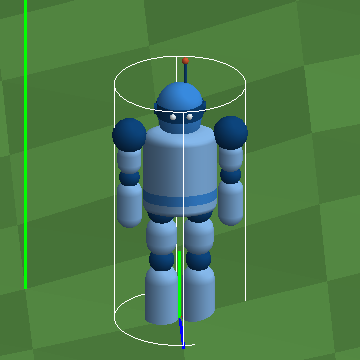
\includegraphics[width=\linewidth]{docs/figures/hw2/ch03_robot-front.png}
        \caption{正面}
    \end{subfigure}\hfill
    \begin{subfigure}[t]{.32\textwidth}
        \centering
        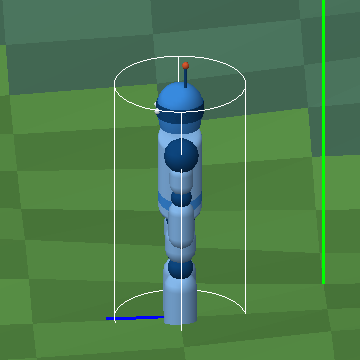
\includegraphics[width=\linewidth]{docs/figures/hw2/ch03_robot-side.png}
        \caption{側面}
    \end{subfigure}\hfill
    \begin{subfigure}[t]{.32\textwidth}
        \centering
        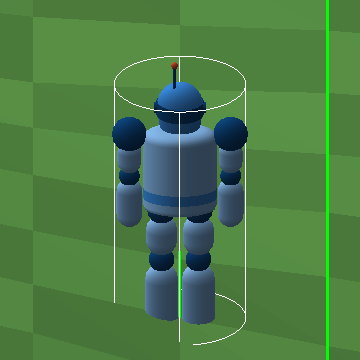
\includegraphics[width=\linewidth]{docs/figures/hw2/ch03_robot-back.png}
        \caption{背面}
    \end{subfigure}
    \caption{機器人的外觀}
    \label{fig:robot-look}
\end{figure}

每個部位都是三角形網格：先用直線、圓弧與 Bézier 曲線在 $x$-$y$ 平面畫出 2D 剖面，
再由 \lstinline|MeshBuilder| 繞 $y$ 軸旋轉成旋轉體（lathe）。

由於純色模型看不出立體表面，因此我參考 Inigo Quilez 的作法，依法向量 $\mathbf{n}$ 與太陽方向 $\mathbf{l}$ 調整亮度。
$\max(0, \mathbf{n} \cdot \mathbf{l})$ 會讓背光面全部同樣暗，所以改將內積映射到 $[0, 1]$ 後平方：
$$
    b(\mathbf{n}) = \left( \tfrac{1}{2}\, \mathbf{n} \cdot \mathbf{l} + \tfrac{1}{2} \right)^2, \qquad
    s(\mathbf{n}) = \min\!\left( 1,\; 0.32 + 0.68 \times 0.9 \times \frac{b(\mathbf{n})}{b(\hat{\mathbf{y}})} \right).
$$
倍率 $s$ 下限為 0.32，避免背光面全黑；平地（$\mathbf{n} = \hat{\mathbf{y}}$）校正為 0.9，讓朝向太陽的斜面仍比平地亮。


\subsection{場景圖}
\label{sec:scene-graph}

機器人的場景圖如圖~\ref{fig:scene-graph}。
每個節點是一根骨頭（bone），記錄它的父節點、關節在父節點座標系中的位置（pivot），以及可轉動的角度範圍。
根節點 root 本身沒有關節，只帶有一個隨姿勢改變的平移量 rootOffset，用來決定髖部離地的高度。
軀幹的原點在髖部中央，雙腿從髖部往下、雙臂從肩膀往下延伸，脖子接在軀幹頂端，頭再接在脖子上。

\begin{figure}[htbp]
    \centering
    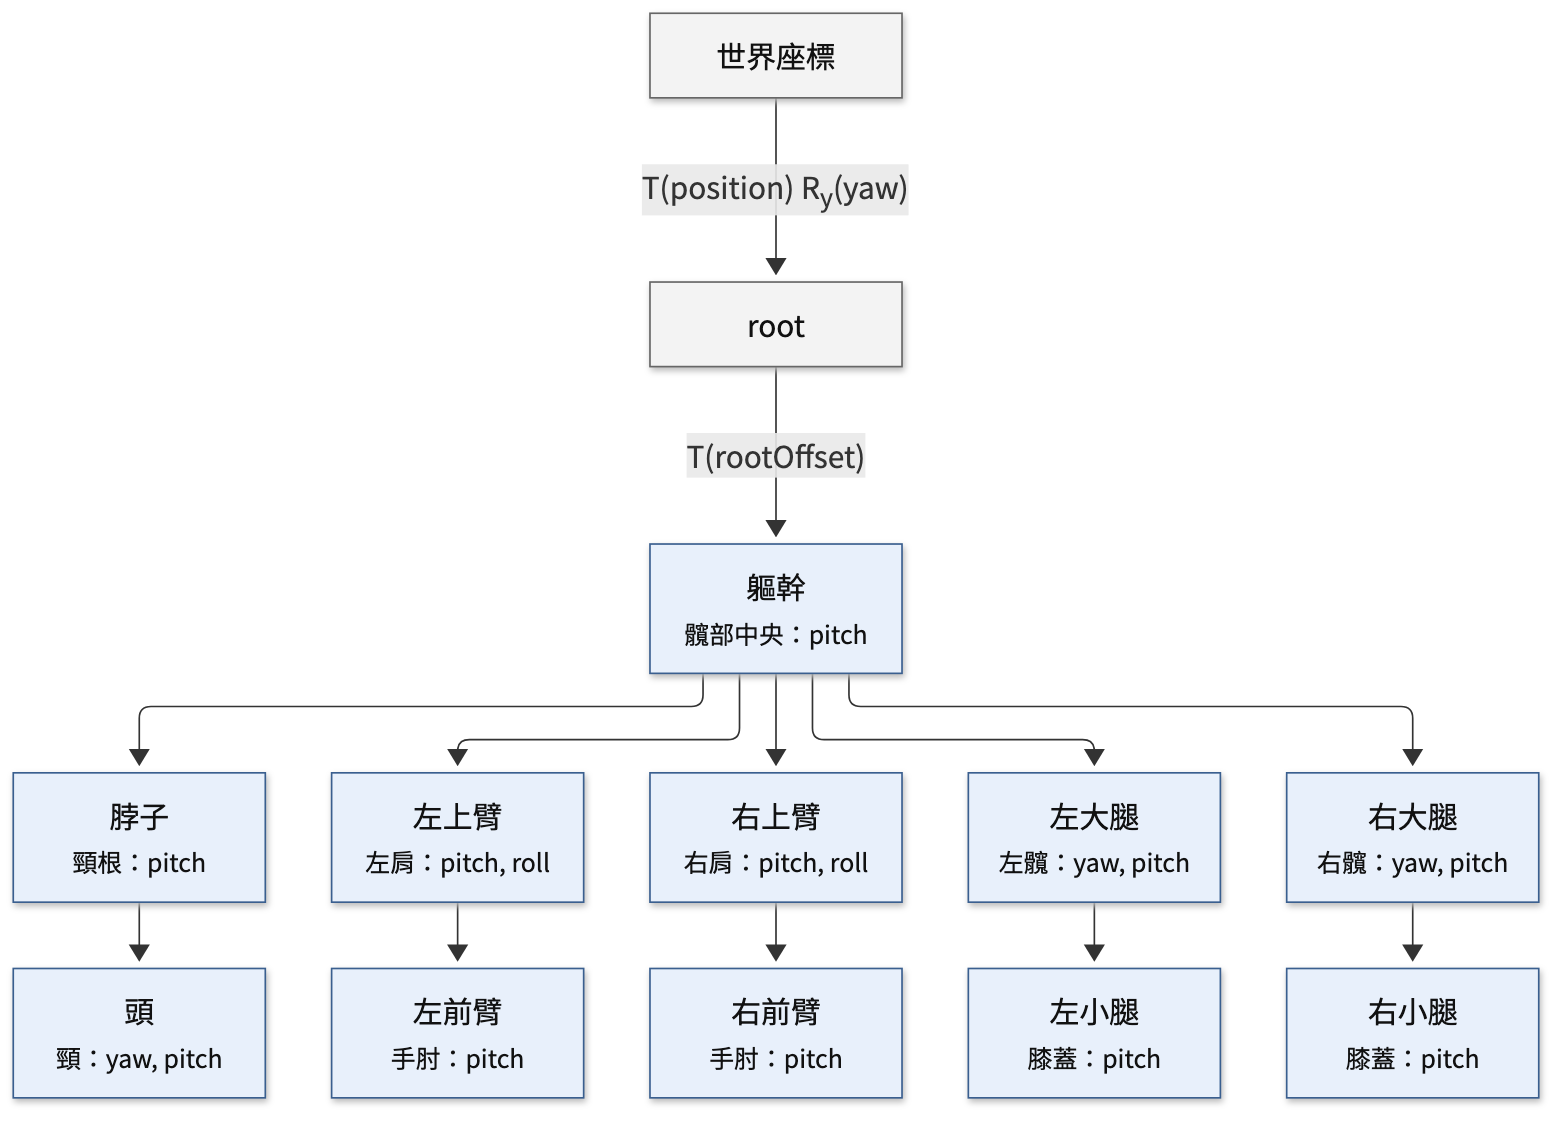
\includegraphics[width=.8\textwidth]{docs/figures/hw2/ch03_scene-graph.png}
    \caption{機器人的場景圖，節點下方為連接父節點的關節與其可轉動的軸}
    \label{fig:scene-graph}
\end{figure}

\subsection{關節自由度}
\label{sec:dof}

每個關節最多有 yaw（繞 $y$ 軸）、pitch（繞 $-x$ 軸）、roll（繞 $z$ 軸）三個旋轉自由度；角度範圍上下限相同的軸視為鎖住，不算一個自由度。
骨頭在靜止姿勢時面向 $+z$，pitch 取 $-x$ 為轉軸，正值就是往前抬起，與視線的 pitch 方向一致。
各關節的自由度與角度範圍如表~\ref{tab:dof}，角度範圍以左側為準，右側的 yaw 與 roll 範圍左右對稱、正負相反。
四肢共有 12 個自由度，加上軀幹、脖子各 1 個與頭部的 2 個，機器人身上共有 16 個旋轉自由度；
另外整隻機器人在世界中還有位置 $(x, y, z)$ 與朝向 yaw 共 4 個自由度。

\begin{table}[H]
    \centering
    \caption{關節的自由度與角度範圍（「—」表示鎖住）}
    \label{tab:dof}
    \small
    \begin{tabular}{lcccc}
        \toprule
        關節       & yaw                       & pitch                      & roll                     & 自由度 \\
        \midrule
        軀幹（髖部中央） & —                         & $-45^\circ \sim 45^\circ$  & —                        & 1   \\
        脖子（頸根）   & —                         & $-45^\circ \sim 45^\circ$  & —                        & 1   \\
        頭（頸）     & $-70^\circ \sim 70^\circ$ & $-60^\circ \sim 50^\circ$  & —                        & 2   \\
        上臂（肩膀）×2 & —                         & $-60^\circ \sim 200^\circ$ & $0^\circ \sim 170^\circ$ & 2   \\
        前臂（手肘）×2 & —                         & $0^\circ \sim 145^\circ$   & —                        & 1   \\
        大腿（髖）×2  & $0^\circ \sim 45^\circ$   & $-30^\circ \sim 120^\circ$ & —                        & 2   \\
        小腿（膝蓋）×2 & —                         & $-140^\circ \sim 0^\circ$  & —                        & 1   \\
        \bottomrule
    \end{tabular}
\end{table}

\subsection{階層繪製}

階層模型的變換順序是先移到關節位置，再套用關節旋轉；所有子節點都會繼承這個變換。
程式用相同順序計算骨頭 $i$ 在機器人模型空間中的矩陣 $M_i$：
$$
    \begin{cases}
        M_{\text{root}} = M_0 = T(\text{rootOffset}), \\
        M_i = M_{\text{parent}(i)} T(\text{pivot}_i)
        R_y(\text{yaw}_i) R_{-x}(\text{pitch}_i) R_z(\text{roll}_i), i \neq \text{root}.
    \end{cases}
$$
骨頭依加入順序儲存，而且父節點一定在子節點之前，因此從頭走過陣列一次就能算完所有矩陣，不需要遞迴。
計算矩陣前，各角度會先限制在表~\ref{tab:dof} 的範圍內，避免姿勢與動畫疊加後超出關節活動範圍。

繪製時先以 \lstinline|glTranslatef|、\lstinline|glRotatef| 移到機器人的位置與朝向，
再對每根骨頭 \lstinline|glPushMatrix|、\lstinline|glMultMatrixf(|$M_i$\lstinline|)|、畫出網格、\lstinline|glPopMatrix|。
由於矩陣採用 OpenGL 的 column-major 排列，可以直接交給 \lstinline|glMultMatrixf|。

這組矩陣也不只用於繪圖。例如，當機器人位於 $\mathbf{p}$、朝向 $\psi$ 時，頭部上的眼睛標記點可由
$$
    \mathbf{p}_{\text{eye,world}} = T(\mathbf{p})R_y(\psi)M_{\text{head}}
    \begin{bmatrix}\mathbf{p}_{\text{eye,local}}\\1\end{bmatrix}
$$
轉成世界座標，作為相機的焦點。

\section{動作與控制}
\label{sec:motion}

\subsection{從輸入到動作}

主迴圈由 \lstinline|glutTimerFunc| 約每 16 ms 觸發一次，依經過時間執行固定 $\frac{1}{60}$ 秒的 tick，最後重畫畫面。
每個 tick 會讀取輸入、更新機器人狀態並進行物理模擬。

按鍵狀態不會直接改變位置，而是先轉成 \lstinline|Intent|。其中記錄前後左右的移動量、跑步與跳躍狀態、要切換的姿勢及視線方向。
機器人每個 tick 依下列順序處理：

\begin{enumerate}
    \item 身體朝向設為視線的 yaw，轉彎因此由視角控制；視線的 pitch 交給頭部關節，超出活動範圍的部分會被截斷
    \item 處理姿勢切換的請求，並推進轉換的進度
    \item 依目前的姿勢決定目標速度，交給物理模擬器計算位移與碰撞（第~\ref{sec:collision} 節）
    \item 以實際移動的距離推進走路的步伐
\end{enumerate}

關節角度等到繪製前才由姿勢與目前步伐算出。輸入端只記錄玩家想做的動作；速度、姿勢限制與碰撞仍由模擬端判斷。

\subsection{姿勢切換}

機器人有站立、潛行與坐下三種姿勢（圖~\ref{fig:stances}）。每種姿勢包含一組關節角度和 rootOffset：
\begin{itemize}
    \item \textbf{站立}：所有關節為 $0^\circ$，髖部高度等於腿長 $L = 13$ px。
    \item \textbf{潛行}：軀幹前傾 $30^\circ$、脖子回抬 $30^\circ$ 讓視線維持水平，大腿往前抬 $60^\circ$、膝蓋彎 $60^\circ$；
          雙腿接在軀幹下會一起前傾，大腿與小腿都和鉛直方向夾 $30^\circ$，因此髖部降到 $\frac{\sqrt{3}}{2} L$。
    \item \textbf{坐下}：大腿往前抬 $90^\circ$ 並向外張開 $15^\circ$，髖部降到大腿厚度的一半，正好坐在地上。
\end{itemize}

切換姿勢固定要花費 0.5 秒。
轉換狀態記錄起點 \lstinline|from|、終點 \lstinline|to| 與進度 $t \in [0, 1]$，所有關節角度和 rootOffset 都依 $t$ 線性內插。
如果途中要求回到原姿勢，程式會交換 \lstinline|from| 與 \lstinline|to|，並將進度改成 $1-t$，讓動作直接從目前位置倒回去。
轉換途中若要求第三種姿勢，輸入會先被忽略，等目前的轉換結束後才能再次切換。
轉換期間不能移動，碰撞箱也會以相同進度改變大小（第~\ref{sec:collision} 節）。

\begin{figure}[htbp]
    \centering
    \begin{subfigure}[t]{.32\textwidth}
        \centering
        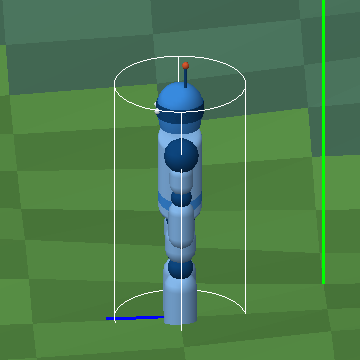
\includegraphics[width=\linewidth]{docs/figures/hw2/ch04_stance-standing.png}
        \caption{站立}
    \end{subfigure}\hfill
    \begin{subfigure}[t]{.32\textwidth}
        \centering
        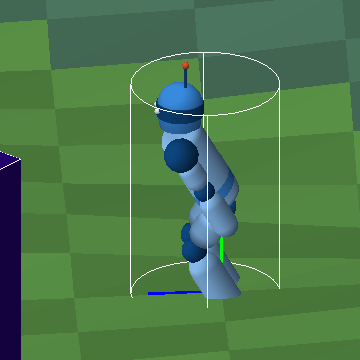
\includegraphics[width=\linewidth]{docs/figures/hw2/ch04_stance-sneaking.png}
        \caption{潛行}
    \end{subfigure}\hfill
    \begin{subfigure}[t]{.32\textwidth}
        \centering
        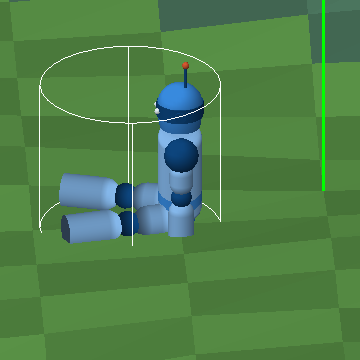
\includegraphics[width=\linewidth]{docs/figures/hw2/ch04_stance-sitting.png}
        \caption{坐下}
    \end{subfigure}
    \caption{三種姿勢；線框為碰撞箱}
    \label{fig:stances}
\end{figure}

\subsection{走路與跑步}

走路動畫參考 Minecraft 的手腳擺動方式，動畫相位是由機器人累積水平移動距離 $d$ 決定：
$$
    \phi = 2\pi \frac{d}{C}, \qquad C = 2 \cdot 2L \sin 25^\circ \approx 1.37 \text{ m},
$$
其中 $C$ 代表左右腳各跨一步的距離。大腿前後各擺 $25^\circ$ 時，兩腳在前後方向相距 $2L\sin25^\circ$，所以一個完整週期取其兩倍。
擺動幅度 $a$ 的目標值為「目前速度／走路速度」，上限為 1.2，停下時則為 0。
另一個係數 $r\in[0,1]$ 表示跑步程度；速度超過走路速度後開始增加，達到兩倍走路速度時為 1。
各關節在站立姿勢上疊加的 pitch 角度為
\begin{align*}
    \text{髖} & = \pm 25^\circ \sin\phi \cdot a,               & \text{膝} & = -40^\circ \max(0, \pm\cos\phi) \cdot a, \\
    \text{肩} & = \mp 20^\circ \sin\phi \cdot a + 180^\circ r, & \text{肘} & = 15^\circ \cdot a \, (1 - r),
\end{align*}
其中 $\pm$、$\mp$ 的上方符號用於身體左側關節、下方用於身體右側關節，pitch 正值為往前抬，因此兩腳交替、手與同側的腳反向擺動。
$\cos\phi$ 的正負代表髖關節角度正在增加或減少，用來區分兩腿的前擺階段。腿從中立位置開始往前擺時膝蓋彎曲，接近前方端點時再逐漸伸直，讓腳尖在擺動期間離地。
當髖關節角度為 $\theta = 25^\circ \sin\phi \cdot a$ 時，rootOffset 會再扣掉 $L(1-\cos\theta)$，使髖部隨步伐上下移動。

跑步時，雙臂會逐漸伸直並舉過頭，再向外張開 $20^\circ r$ 成 V 字。
$a$ 與 $r$ 不會立刻跳到目標值，而是在每個 tick 以 $x \leftarrow x + (x^\ast - x)(1 - e^{-k\,\Delta t})$ 逼近。
因此起跑與停下時，四肢會逐漸展開或回到原位。

\subsection{跳躍與重力}

重力使用半隱式 Euler 法積分，每個 tick 先更新速度，再用新速度更新位置：
\begin{equation*}
    \mathbf{v} \leftarrow \mathbf{v} + \mathbf{a} \Delta t, \qquad
    \mathbf{x} \leftarrow \mathbf{x} + \mathbf{v} \Delta t, \qquad
    \mathbf{a} = [0, -g, 0],\; g = 9.80665 \text{ m/s}^2 .
\end{equation*}
著地時假設摩擦力足夠大，水平速度可直接改成目標速度。離地後只受重力影響，因此會保留起跳瞬間的水平速度，無法在空中改變移動方向或速度。
設定目標跳躍高度 $h=0.5$ m，再由連續時間的關係 $v^2=2gh$ 算出鉛直起跳速度 $v_y=\sqrt{2gh}$。實際位置以固定時間步長積分，因此模擬得到的最高點會有些微離散誤差。

\subsection{動作限制}

\begin{itemize}[nosep]
    \item \textbf{速度}：站立時走路 1.2 m/s、跑步 3 m/s，潛行 0.6 m/s，坐下或轉換姿勢時為 0；
          前後與左右同時按下時，合成方向的長度會被限制在 1，斜走不會比直走快。
    \item \textbf{關節角度}：每次計算骨架矩陣前，所有角度都會被截斷到表~\ref{tab:dof} 的範圍。
    \item \textbf{姿勢}：只有站立能跑，坐下不能移動或跳躍；跳躍還需雙腳著地。
\end{itemize}

\section{碰撞偵測}
\label{sec:collision}

\subsection{碰撞形狀}

機器人的碰撞箱是以腳底中心為基準的直立圓柱；障礙物有可繞 $y$ 軸旋轉的方塊、直立圓柱與球。
除了球以外的形狀都是直立的，因此鉛直與水平重疊可以分開計算。

圓柱尺寸取自各姿勢實際占用的範圍（圖~\ref{fig:stances} 線框）：
站立時半徑 0.45 m、高 1.75 m；潛行時 0.51 m、1.57 m；坐下時 0.61 m、1.06 m。
後兩者的中心分別前移 0.11 m 與 0.34 m 以包住前伸的腿，偏移隨身體朝向旋轉，切換姿勢時也一起內插。

\subsection{偵測與推擠}

每個 tick 先依速度移動碰撞箱，再檢查周圍 $3\times3$ 個 chunk 中的障礙物。
偵測函式會回傳接觸法線 $\mathbf{n}$ 與穿透深度 $\delta$，三種形狀分別以下列方式計算：
\begin{itemize}[nosep]
    \item \textbf{方塊}：把圓柱中心轉到方塊的局部座標，將中心夾在方塊的 $x$、$z$ 範圍內得到最近點，最近點到圓心的距離小於半徑即為碰撞。
          若圓心已位於方塊的水平範圍內，則改用距離最近的邊界決定推出方向，穿透深度為圓心到該邊界的距離再加上圓柱半徑。
    \item \textbf{圓柱}：兩圓心的水平距離小於半徑和即為碰撞。
    \item \textbf{球}：在圓柱上找離球心最近的點（高度夾在圓柱上下緣之間，水平方向夾在圓周內），距離小於球的半徑即為碰撞。
\end{itemize}
水平與鉛直重疊量算出後，選擇較小的一項作為推出方向。例如從方塊上方落下時，通常是鉛直重疊較小，機器人便會被向上推出並停在頂面。

以 $\mathbf{n}$ 表示由機器人指向障礙物的單位法線，碰撞時修正為
$$
    \mathbf{x} \leftarrow \mathbf{x}-\delta\mathbf{n}, \qquad
    \mathbf{v} \leftarrow \mathbf{v}-\max(0,\mathbf{v}\cdot\mathbf{n})\mathbf{n}
$$
即只移除朝向障礙物的速度分量，保留沿表面的分量，斜撞牆面時仍可沿牆滑動。
推出可能造成新的重疊，所以每個 tick 最多重複 5 次；表面相切也算深度 0 的接觸，站在障礙物上時才不會反覆離地。

\subsection{陡坡與支撐面}

地形由三角形組成，任一水平位置都能查到高度與法向量。當法向量和 $y$ 軸的夾角小於 $45^\circ$（$n_y>\frac{\sqrt{2}}{2}$）時，該表面可以行走。
更陡的坡面視為牆壁；若腳底低於坡面，就沿法向量的水平分量向外推出，距離為高度差乘上 $\cot$（坡度），使機器人無法繼續爬升。

完成推擠後，程式會在腳底下方搜尋支撐面，取可行走地形與朝上障礙物頂面中最高的一個。腳底碰到支撐面即判定為著地。
另外，如果上一個 tick 已經著地、目前沒有向上跳，而且離支撐面不超過 0.3 m，機器人會直接貼回表面。
這項處理是為了解決下坡時每一步都短暫離地，導致移動控制失效的問題。

\section{世界生成}
\label{sec:world}

\subsection{地形與 Chunk}

原本的作業規格使用 $[0,0,0]$ 到 $[50,0,50]$ 的平面。我將地板改成依 seed 生成的起伏地形，並切成邊長 16 m 的 chunk。
程式只保留機器人周圍半徑 12 個 chunk，移動時會釋放遠處區塊並生成新區塊，因此地形可以持續向外延伸（圖~\ref{fig:terrain}）。

地形高度由自行實作的 Perlin noise 與 fBm 產生，再依高度與環境參數決定地表顏色。
各 chunk 的內容由世界 seed 和座標決定，相同 seed 會得到相同結果。地形網格只在 chunk 第一次繪製時建立並快取，避免每幀重新取樣雜訊。

\subsection{障礙物}

每個 chunk 預先選定三個位置，分別嘗試放置方塊、球與圓柱；若位置位於水面或冰面則不生成。
方塊的長寬高與旋轉角度、球的半徑、圓柱的半徑與高度都由位置 seed 決定，尺寸上限為 2 m，顏色也使用同一 seed 產生。
障礙物底部貼齊當地地面，並和地形一樣轉成網格繪製，再套用第~\ref{sec:robot} 節依法向量計算的明暗效果。

\begin{figure}[htbp]
    \centering
    \begin{subfigure}[t]{.48\textwidth}
        \centering
        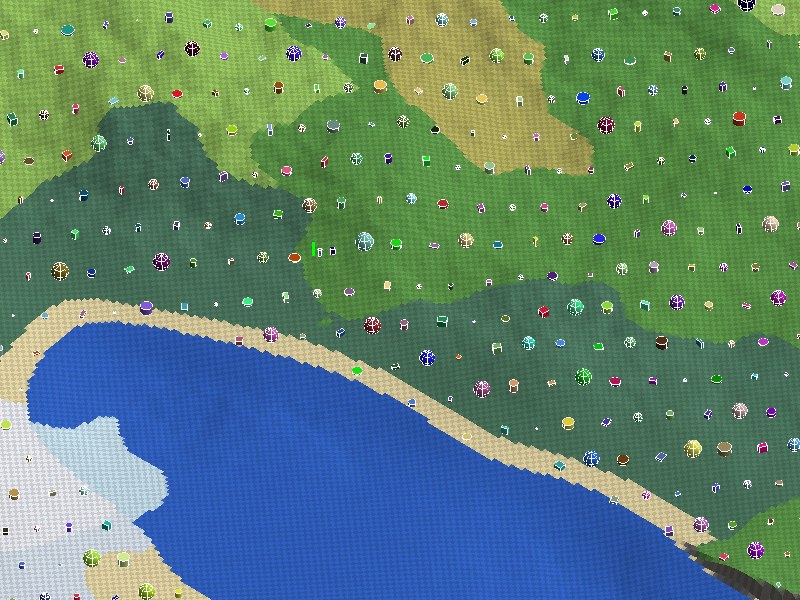
\includegraphics[width=\linewidth]{docs/figures/hw2/ch06_terrain.png}
        \caption{地形與生態系概觀}
    \end{subfigure}\hfill
    \begin{subfigure}[t]{.48\textwidth}
        \centering
        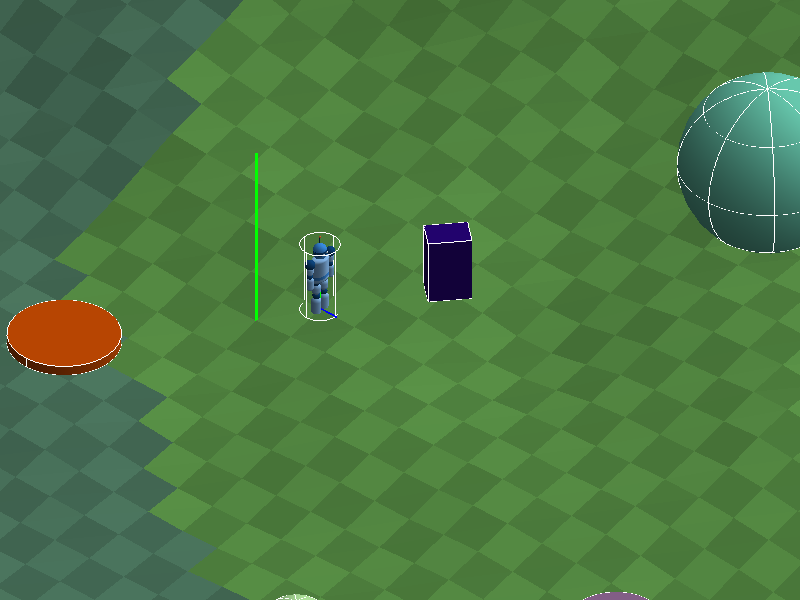
\includegraphics[width=\linewidth]{docs/figures/hw2/ch06_obstacles.png}
        \caption{方塊、球與圓柱障礙物}
    \end{subfigure}
    \caption{地形與障礙物}
    \label{fig:terrain}
\end{figure}

\section{心得}

這是我第一次設計需要隨時間連續更新狀態的即時互動程式。過去寫的網頁服務只需等待請求再處理事件；
這次即使沒有輸入，機器人和世界仍要在每個 tick 持續更新，原本習慣的事件處理方式很快就讓輸入、動畫和繪圖混在一起。

為了整理架構，我參考 Minecraft 等遊戲的作法，逐步拆分輸入、模擬和繪製，機器人也改成將骨架、姿勢和外觀分開保存。
中途改過很多次，有些部分甚至推翻重做，但當站立、潛行、跑步和碰撞陸續加進來時，我才感覺架構開始能承受功能的增加。

這次最有成就感的是從零實作 Perlin noise：依序完成格點梯度、內積、平滑內插與 seed 處理，再疊加成 fBm 生成地形。
看到相同 seed 產生相同世界、分開生成的 chunk 也能無縫接合時，我覺得花的時間很值得。
地形原本不是作業重點，卻是我投入最多心力、也最滿意的部分。


\end{document}
